\chapter{Hardware Implementation}
\label{Chapter 4}
\lhead{Chapter 4. \emph{Hardware Implementation}}

To help demonstrate the usefulness of the stack in a practical manner, a robot was designed and constructed. This robot, named the \emph{ExplorerBot}, was then used to give a practical reference implementation of a full project utilizing the custom embedded Bluetooth stack in a real-world environment.

\section{Hardware Overview}

The completed robot design for the project contains many useful capabilties for both mobility and exploration. Built on top of a pre-fabricated (including raw DC motors and gearing) "Tank" style hobby robot base, the \emph{ExplorerBot} robot implements the following features:

\begin{itemize}
	\item Primary switch-mode based 5V power supply
	\item Secondary LDO based 3.3V power supply for attached sensors
	\item 2x16 Alphanumeric LCD Screen for feedback to the user
	\item Two momentary pushbuttons for user control
	\item One RGB status LED for basic status feedback
	\item Dual PWM motor control system, with variable speed and direction of DC motors
	\item Level converted I\textsuperscript{2}C bus for the attached sensor(s)
	\item Support for the Atmel \textit{Inertial One} and \textit{Pressure One} sensor boards
	\item High intensity LED based headlights for frontal illumination
	\item Piezo speaker for audio feedback and "horn" like functionality
	\item Atmel \textit{AT90USB1287} 8-Bit Microcontroller
	\item External 128KB SRAM for temporary storage of packets to and from the Bluetooth adapter
\end{itemize}

The complete robot design was created in the \textit{Altium Designer} software, including both the schematic design and board routing. Surface mount components were chosen where possible to reduce the board space required, and two board layers used as this proved to offer the lowest cost/time ratio. The final board design measured 10cm x 15cm, however much of this board space is relatively unused; with optimization, this board space could be reduced considerably.

To get the best results in the construction of the robot, the boards were manufactured commercially. This process ensured the manufactured board's quality while also provided solder mask and silkscreen to reduce the potential for error in the robot's construction.

\section{Hardware Modules}

In the section, the various hardware components of the constructed robot are detailed at the block level. Figure \ref{fig:robotblockhw} below illustrates how the various hardware blocks that comprise the robot connect together to make the final design.

\vspace{1em}

\begin{figure}[H]
	\centering
		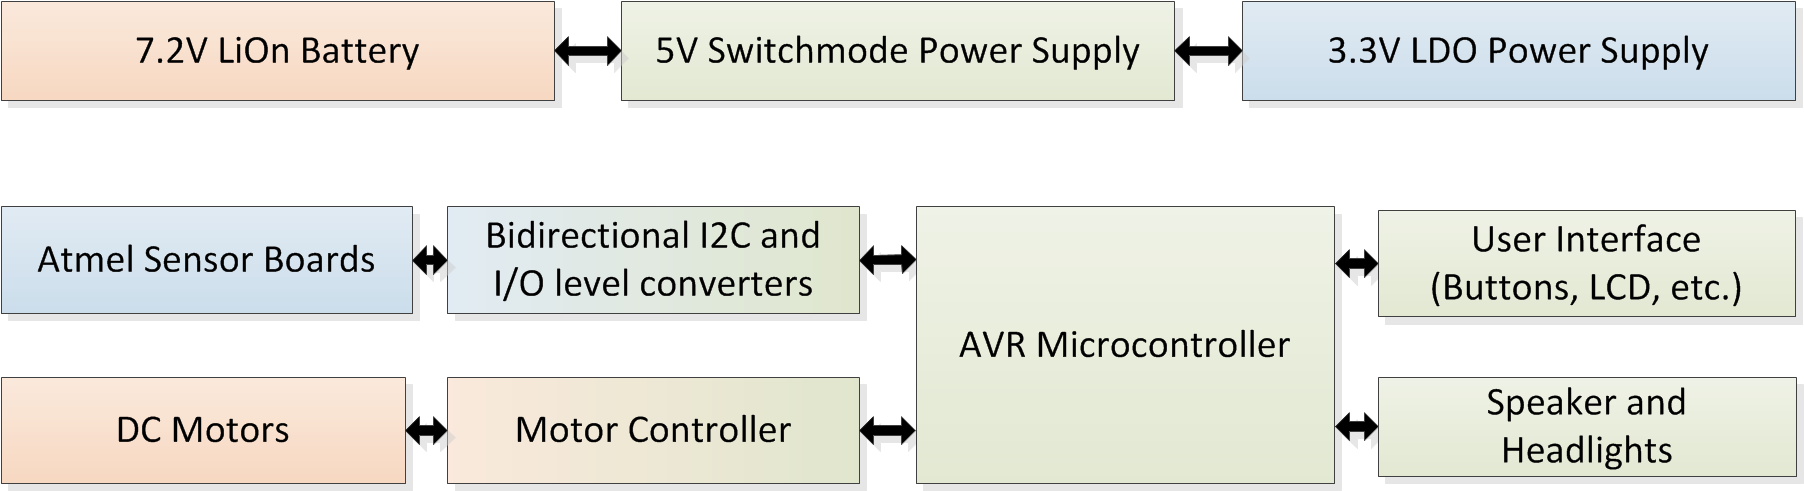
\includegraphics[width=140mm]{./Figures/BlockDiagram.png}
	\rule{35em}{0.5pt}
	\caption[Hardware Block Diagram]{Robot Hardware Block Diagram}
	\label{fig:robotblockhw}
\end{figure}

\subsection{Microprocessor}

Due to the author's familiarity with the Atmel line of \textit{AVR} branded microcontrollers, one of the avaliable models in this line-up was chosen to serve in the robot as the main processor, the AT90USB1287. This 8-bit microcontroller contains 128KB of non-voltatile FLASH memory for program storage, 4KB of non-voltatile EEPROM for user application parameter storage and 8KB of internal SRAM for scratch memory. A 16MHz clock (provided by an external crystal) was selected for the design as this offered the fastest possible speed the chip was capable of, while still allowing the hardware USB host controller inside the chip to function normally. As a trade-off, this higher clock speed put a constraint on the main logic level voltage; at 16MHz, the AVR microcontroller required 5V to be within the datasheet's specifications.

As the AT90USB1287 and associated USB components are difficult to source in single quantities at reasonable prices, the use of a commercial breakout module containing this chip was selected instead: the \textit{Micropendous-A} board (see Figure \ref{fig:micropendous}). This board contains the surface mount AVR microcontroller and associated USB components, along with an external 128KB SRAM chip attached to the AVR's external memory bus interface. As the Bluetooth stack required a large temporary buffer for incoming fragments, the selection of this board proved ideal for the intended purpose.

\begin{figure}
	\centering
		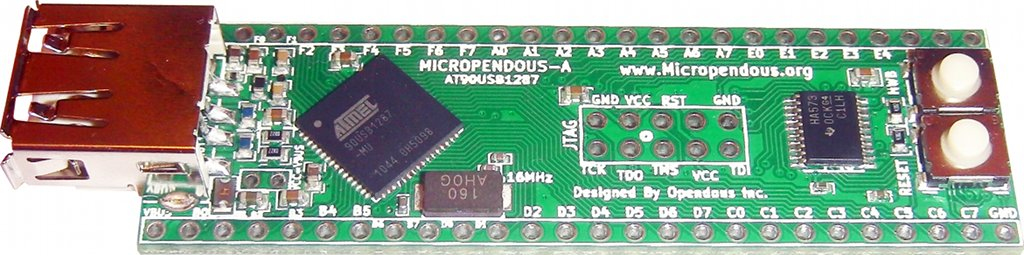
\includegraphics[width=100mm]{./Figures/MicropendousA.jpg}
	\rule{35em}{0.5pt}
	\caption[Micropendous-A Board]{The Micropendous-A Board (Image courtesy \textit{Opendous Inc.})}
	\label{fig:micropendous}
\end{figure}

\subsection{Primary Power Supply}

As the vast majority of the robot's hardware operated at a fixed 5V level, a power supply was required to reduce the Lithium Ion battery's raw 7.2V (nominal) voltage down to the 5V level needed to power the various components. Due to the use of battery power in the project, reducing power consumption where possible was a large concern; thus, a switchmode design was chosen for maximum voltage conversion efficiency. A conventional linear regulator was considered for the design, but rejected due to the prohibitably large amount of power this would waste (approximately .45W, assuming an average 200mA operating current).

The regulator selected for the project was the M2595S-5.0, a fixed-function switchmode regulator capable of outputing a fixed 5V rail at loads of up to 3A. While the robot design would not consume even a fifth of this power, the overhead ensured that the power supply would remain robust and the output within the tollerances of the system components regardless of the load demanded. The exact schematic used in the final robot power supply design was taken from the regulator component's datasheet to ensure correct operation.

% TODO - diagrams showing layout and schematic of power supply

\subsection{User Interface}

For interaction with the user, the robot contains several components, detailed below.

\subsubsection{RGB Status LED}

For primary status indication, a surface mount RGB LED indicates the current status of the robot. Due to a lack of free PWM channels on the AVR microcontroller, the three LED subcomponents are wired directly to standard GPIO ports. While this prevents PWM fading from producing a many-bit custom colour from the LED, a three bit colour space is possible giving a total of 7 possible colours (and no colour when all the LED subcomponents are turned off). For the purposes of the created robot, this is in practice more than enough for basic status indication.

To achieve a somewhat uniform brightness, the three LEDs were adjusted with current limiting resistors to consume an equal amount of current (approx. 5mA) despite differing forward voltages. As the RGB status LED shares the same I/O pins as the microcontroller's JTAG port for programmign and debugging, the RGB LED's common annode was connected via a removable wire link to ensure that it could be taken out-of-circuit if it proved to intefere with the external hardware debugger during development.

\subsubsection{LCD Display}

For situations where more information needs to be communicated to the user than is possible via the RGB status LED, a 16x2 Alphanumeric LCD display - compatible with the well known Hitatchi HD44780 chipset - was added to the design. Due to the limited number of GPIO pins avaliable on the microcontroller, the LCD was wired in 4-bit mode, with the lower 4 data pins on the LCD being wired directly to ground. While this doubled the time required to send a byte to the LCD (as bytes then need to be split into a pair of 4-bit nibbles) the high speed of the processor meant that in practice this had little or no effect to the overall speed of the system.

The LCD backlight was wired through a driver transistor to a spare PWM channel on the AVR microcontroller, allowing for 8-bit PWM brightness control to reduce power consumption of the backlight when not in use.

\subsubsection{Buttons}

A pair of standard PCB round buttons were added to the design, for user input. These buttons were wired directly to the microcontroller's GPIO pins; internal pull-up resistors in the microcontroller takes care of maintaining a defined logic level on the pins when the buttons are released, while software handles the debouncing of the button signals.

\subsection{Headlights}

To provide illumination of the area immediately ahead of the robot, a pair of high intensity white LEDs were added to the schematic, connected to a single common driver transistor and driven by a GPIO pin of the microcontroller. To ensure maximum illumination, the LEDs were driven at just under their full 20mA rating when turned on. These "headlights" were then mounted on the front of the robot chassis.

\subsection{Speaker}

A small PCB Piezo speaker was added to the robot, in order to provide both audio feedback for important events (such as Bluetooth connections and disconnections) as well as to act as a miniature horn to attract the attention of any organic obstacles to encourage then to move away from the robot's line of motion. Rather than mounting the speaker directly onto the PCB, it was determined that a better location was in between the two frontal headlight LEDs, with the speaker then connected back to the PCB via flyleads. This arrangement made the directional speaker point in the orientation most suited to a car horn, i.e. towards the front of the robot.

To drive the speaker, a standard NPN transistor was employed to provide sufficient current, driven from an 8-bit PWM timer output GPIO pin of the AVR microcontroller.

\subsection{Motor Controller}

% TODO

\subsection{Sensors}

To provide a measure of feedback from the robot, a number of sensors were added to the design. These sensors, when attached, would allow for the robot's environment to be logged and (potentially) reacted to.

\subsubsection{Sensor Power Supply}

While the main system logic and user interface components run from the main switch-mode 5V power supply, the sensor boards were required to run at a fixed 3.3V level, without the possibility of conversion to suit the higher rail voltage.

For this reason, and to reduce the amount of noise on the sensor power supply for maximum precision, a desision was made to add a secondary power supply, running from the 5V rail, to step down the voltage to the 3.3V required by the sensor boards. For best results, an ADP3308 Low Dropout (LDO) style regular was used as this provided both low output rail noise and minimal wasted power.

\subsubsection{Level Converters}

Due to the differing bus voltages between the sensor boards (3.3V) and the main processor (5V), level conversion of the I\textsuperscript{2}C bus and sensor interrupt/control lines was required. While only a unidirectional buffer was strictly needed for each of the sensor interrupt/control lines, it was decided to use a bidirectional converter to ease the board routing.

Initially, only an ADG3308 8-channel Bidirectional Level Converter IC was used, for both the sensor interrupt/control lines, as well as the I\textsuperscript{2}C bus. However, after further analysis it was discovered that the level translater would not meet the timing requirements of the I\textsuperscript{2}C bus, neccesitating the addition of a secondary dedicated Texas Instruments PCA9306 fixed function I\textsuperscript{2}C bus level converter IC in the second revision of the board. As a bonus, the use of the later chip allowed the I\textsuperscript{2}C bus to be driven at the "Fast" I\textsuperscript{2}C speed of 200KHz for minimal latency and maximum throughput.

The board routing complexity was reduced slightly by swapping the functions of the PCA9306 bus level translatator's SDA and SCL pins on both sides of the IC; this modification (allowable as indicated in the device's datasheet) prevented the need to introduce additional board vias and longer trace routes.

% TODO - schematic showing swapped pin functions

\subsubsection{Atmel Sensor Boards}

By designing the robot around a pair of commercially available Atmel sensor boards for environmental feedback, the design of the robot was considerably simplified and the total unit cost lowered. The \textit{Atmel Pressure One} board contains a Bosch BMP085 Pressure Sensor IC for air pressure sensing, while the Atmel \textit{Inertial One} contains a 3-Axis ITG3200 Gyroscope, 3-Axis BMA150 Accelerometer and 3-Axis AK8975 Compass IC (see Figure \ref{fig:atmelsensorboards}). As several of the sensors also contain a digital temperature sensor in addition to the primary sensor (for calibration and stability feedback) this functionality was also used by the robot to measure the environmental temperature in real time.

Each sensor IC is driven by the main microcontroller of the robot over the level converted I\textsuperscript{2}C bus and one or more interrupt/control lines.

\begin{figure}
	\centering
		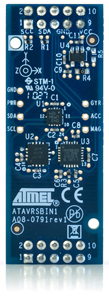
\includegraphics[height=70mm]{./Figures/Inertial1.jpg}
		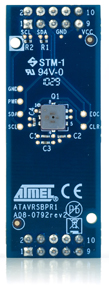
\includegraphics[height=70mm]{./Figures/Pressure1.jpg}
	\rule{35em}{0.5pt}
	\caption[Atmel Sensor Boards]{The Atmel \emph{Inertial One} (left) and \emph{Pressure One} (Right) Sensor Boards (Image courtesy \textit{Atmel Corp.})}
	\label{fig:atmelsensorboards}
\end{figure}

